\documentclass[tikz,border=9pt]{standalone}
\usepackage{amsmath,amssymb}
\usepackage{xcolor}
\usepackage{braket}
\usetikzlibrary{calc,positioning}

\colorlet{linecol}{black}
\colorlet{blockfill}{white}
\colorlet{textcol}{black}

\tikzset{
  wire/.style={draw=linecol, line width=0.4pt},
  block/.style={draw=linecol, line width=0.4pt, fill=blockfill,
                minimum width=4.2cm, minimum height=2.2cm},
  lab/.style={font=\small\rmfamily, text=textcol},
  mathlab/.style={font=\normalsize, text=textcol},
}

\begin{document}
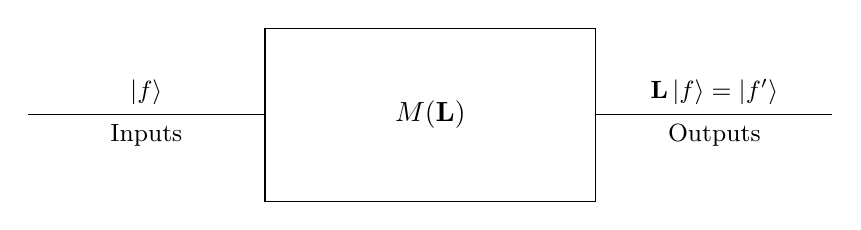
\begin{tikzpicture}[x=1cm,y=1cm]

  % Central block
  \node[block] (B) at (0,0) {};
  \node[mathlab] at (B) {$M(\mathbf{L})$};

  % Left and right wires with endpoints for labels
  \path (B.west) -- ++(-3,0) coordinate (Lend);
  \path (B.east) -- ++(3,0)  coordinate (Rend);

  \draw[wire] (Lend) -- (B.west);
  \draw[wire] (B.east) -- (Rend);

  % Midpoints for annotating
  \path let \p1=($(B.west)!0.5!(Lend)$),
           \p2=($(B.east)!0.5!(Rend)$) in
    node[lab, above] at (\p1) {$\ket{f}$}
    node[lab, below] at (\p1) {Inputs}
    node[lab, above] at (\p2) {$\mathbf{L}\ket{f}=\ket{f'}$}
    node[lab, below] at (\p2) {Outputs};

\end{tikzpicture}
\end{document}